\chapter{Situation de départ - Hardware}

\section{Présentation de la maquette}
La maquette est constituée de cinq PCB, soit une carte principale et quatre cartes de puissance, ainsi que de quatre inducteurs, comme illustré sur les figures \ref{fig:MaquetteUp} et \ref{fig:MaquetteSide}.

\begin{figure}[H]
    \centering
    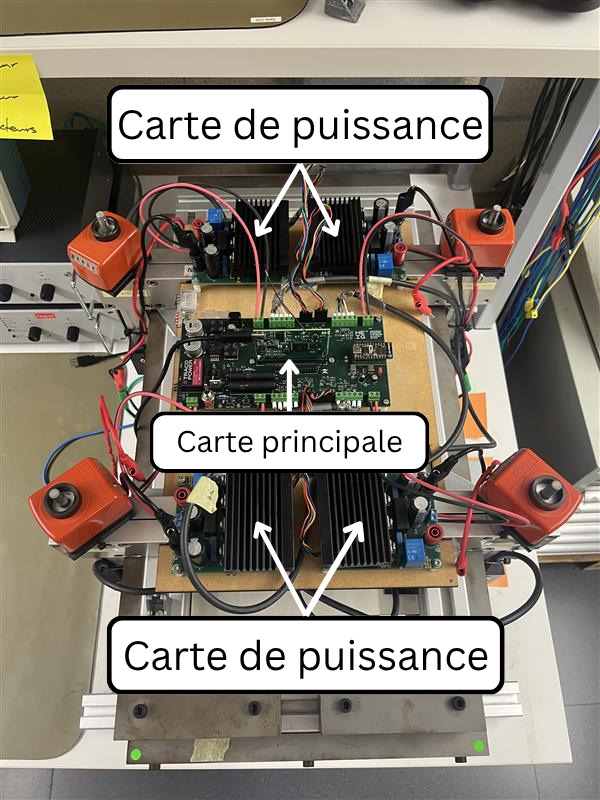
\includegraphics[width=0.6\linewidth]{assets/Chap2/MaquetteDessus.png}
    \caption{La maquette vue de dessus}
    \label{fig:MaquetteUp}
\end{figure}

\begin{figure}[H]
    \centering
    
\includegraphics[width=1\linewidth]{assets/Chap2/MaquetteCote.png}
    \caption{La maquette vue de côté}
    \label{fig:MaquetteSide}
\end{figure}

Comme présenté sur les images \ref{fig:MaquetteUp} et \ref{fig:MaquetteSide}, la maquette comprend :
\begin{itemize}
    \item une carte principale.
    \item quatre cartes de puissance.
    \item quatre inducteurs.
    \item quatre capteurs de courant.
    \item quatre capteurs de position.
\end{itemize}

Une symétrie est réalisée afin de permettre aux inducteurs d’avoir une répartition de masse équilibrée.

Les différentes dimensions, exprimées en $mm$, de la partie lévitante de la maquette sont représentées sur l’image \ref{fig:TailleMaquette} :

\begin{figure}[H]
    \centering
    \includesvg[width=1\linewidth]{assets/Chap2/MaquetteTaille}
    \caption{Dimension de la partie lévitante de la maquette}
    \label{fig:TailleMaquette}
\end{figure}

Les éléments numérotés ci-dessous sont les suivants :
\begin{enumerate}
    \item Le capteur de position.
    \item L’inducteur, au nombre de 4.
    \item Le rail.
    \item La plaque en bois stratifié blanc servant de référence aux capteurs de positions
    \item La pièce assurant le maintien sur le pied et sur la partie supérieure.
    \item La partie supérieure contenant l’électronique.
\end{enumerate}

La partie supérieure et la partie inférieure assemblées constituent l’ensemble lévitant. À la suite d’une mesure de masse, la partie lévitante ne pèse pas 13,6 kg, comme indiqué dans les travaux précédents, mais 18,052 kg.

Les inducteurs présentent une résistance de $0,8\text{ }\Omega$ et comportent chacun 125 spires. La surface des entrefers sont de $1000\text{ }mm^2$ ($50\text{ }mm\text{ }x\text{ }20\text{ }mm$).

\begin{figure}[H]
    \centering
    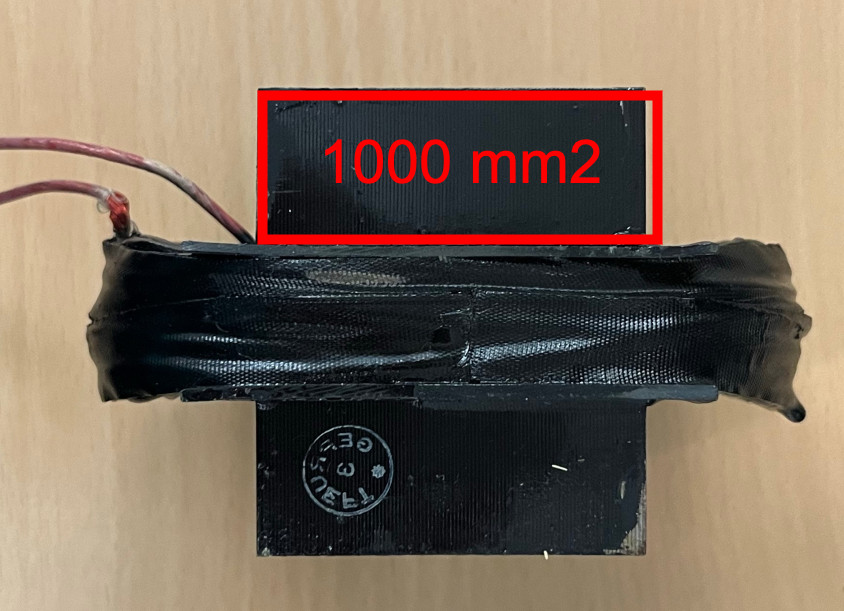
\includegraphics[width=0.5\linewidth]{assets/Chap2/inducteur.jpg}
    \caption{Surface d'un seul inducteur}
    \label{fig:surface_inducteur}
\end{figure}

Les capteurs de courant sont des capteurs LEM \cite{CaptCour}. Il s’agit de capteurs à effet Hall. Ces capteurs sont disposés sur les cartes de puissance. Leur plage de mesure s’étend de $-30\text{ }A$ à $30\text{ }A$ (voir tracé \ref{fig:GrapheCaptCour}). Leur bande passante est de $50\text{ }kHz$. Ils permettent de mesurer le courant traversant les bobines.

\begin{figure}[H]
    \centering
    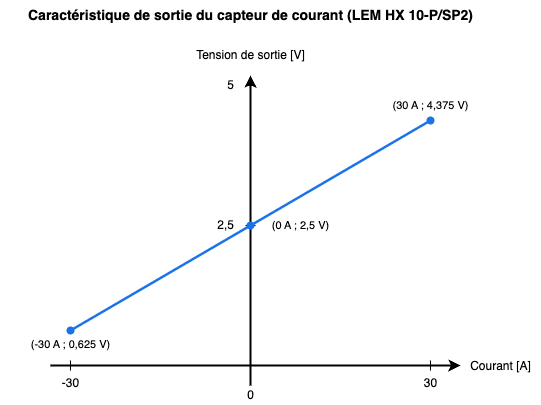
\includegraphics[width=0.75\linewidth]{assets/Chap2/CaracteristiqueCourant.png}
    \caption{Caractéristique de sortie du capteur de courant}
    \label{fig:GrapheCaptCour}
\end{figure}

Les capteurs de position sont des capteurs Baumer \cite{CaptPosition}. Il s’agit de capteurs optiques par triangulation laser. Leur distance de base se situe entre $30\text{ }mm$ et $70\text{ }mm$ (voir tracé \ref{fig:GrapheCaptPos}). Grâce à une fonction d’apprentissage, cette plage peut être réduite afin de se focaliser sur la distance de l’entrefer. Afin de réaliser une calibration du capteur, il est possible de suivre les instructions de la \autoref{sec:CalibrationCaptPos}.

\begin{figure}[H]
    \centering
    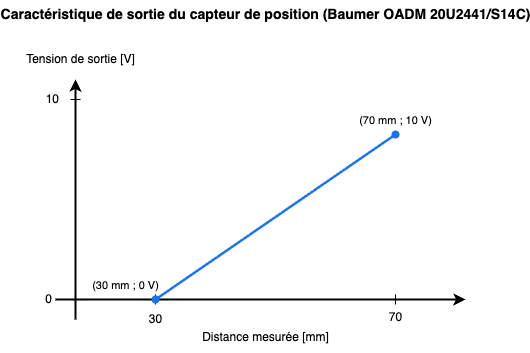
\includegraphics[width=0.75\linewidth]{assets/Chap2/CaracteristiquePosition.png}
    \caption{Caractéristique de sortie du capteur de position}
    \label{fig:GrapheCaptPos}
\end{figure}

De plus amples détails sur l’électronique sont présentés dans la section \ref{sec:SchemEle}.

\clearpage

\section{Schéma fonctionnel}
Le schéma fonctionnel de la maquette est présenté ci-dessous :

\begin{figure}[H]
    \centering
    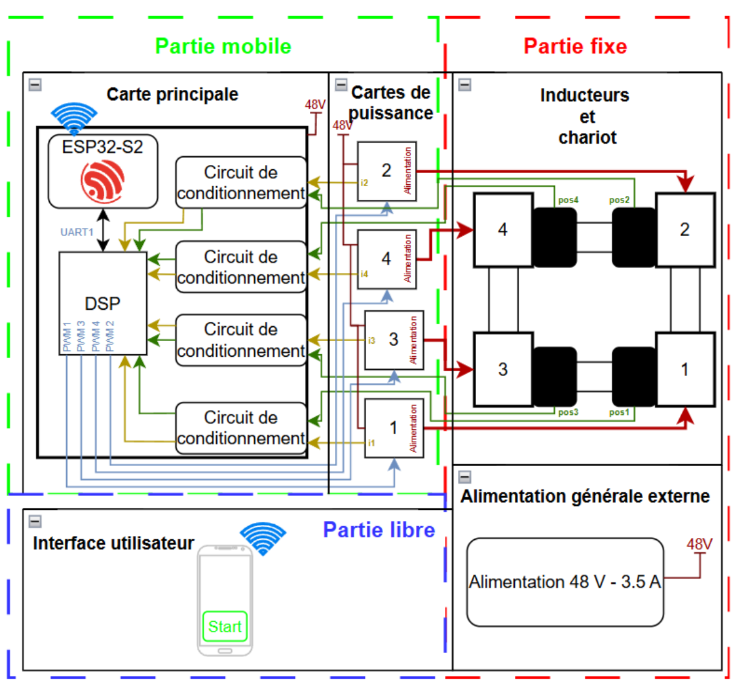
\includegraphics[width=1\linewidth]{assets/Chap2/SchemFonct.png}
    \caption{Schéma fonctionnel}
    \label{fig:SchemFonct}
\end{figure}

Sur le principe, la carte principale doit assurer l’ensemble de la régulation. Elle permet donc de commander les inducteurs pour la lévitation.

La maquette peut être commandée à l’aide d’une interface web accessible depuis un téléphone ou tout autre appareil pouvant se connecter au réseau Wi-Fi de l’ESP32.

Actuellement, une alimentation de laboratoire est utilisée. À terme, l’intégration d’une alimentation propre au système sera mise en place.

\clearpage

\section{Présentation de l'électronique}
\label{sec:SchemEle}
La section suivante présente l’électronique réalisée au départ du projet. Le schéma électrique complet est le suivant :

\begin{figure}[H]
    \centering
    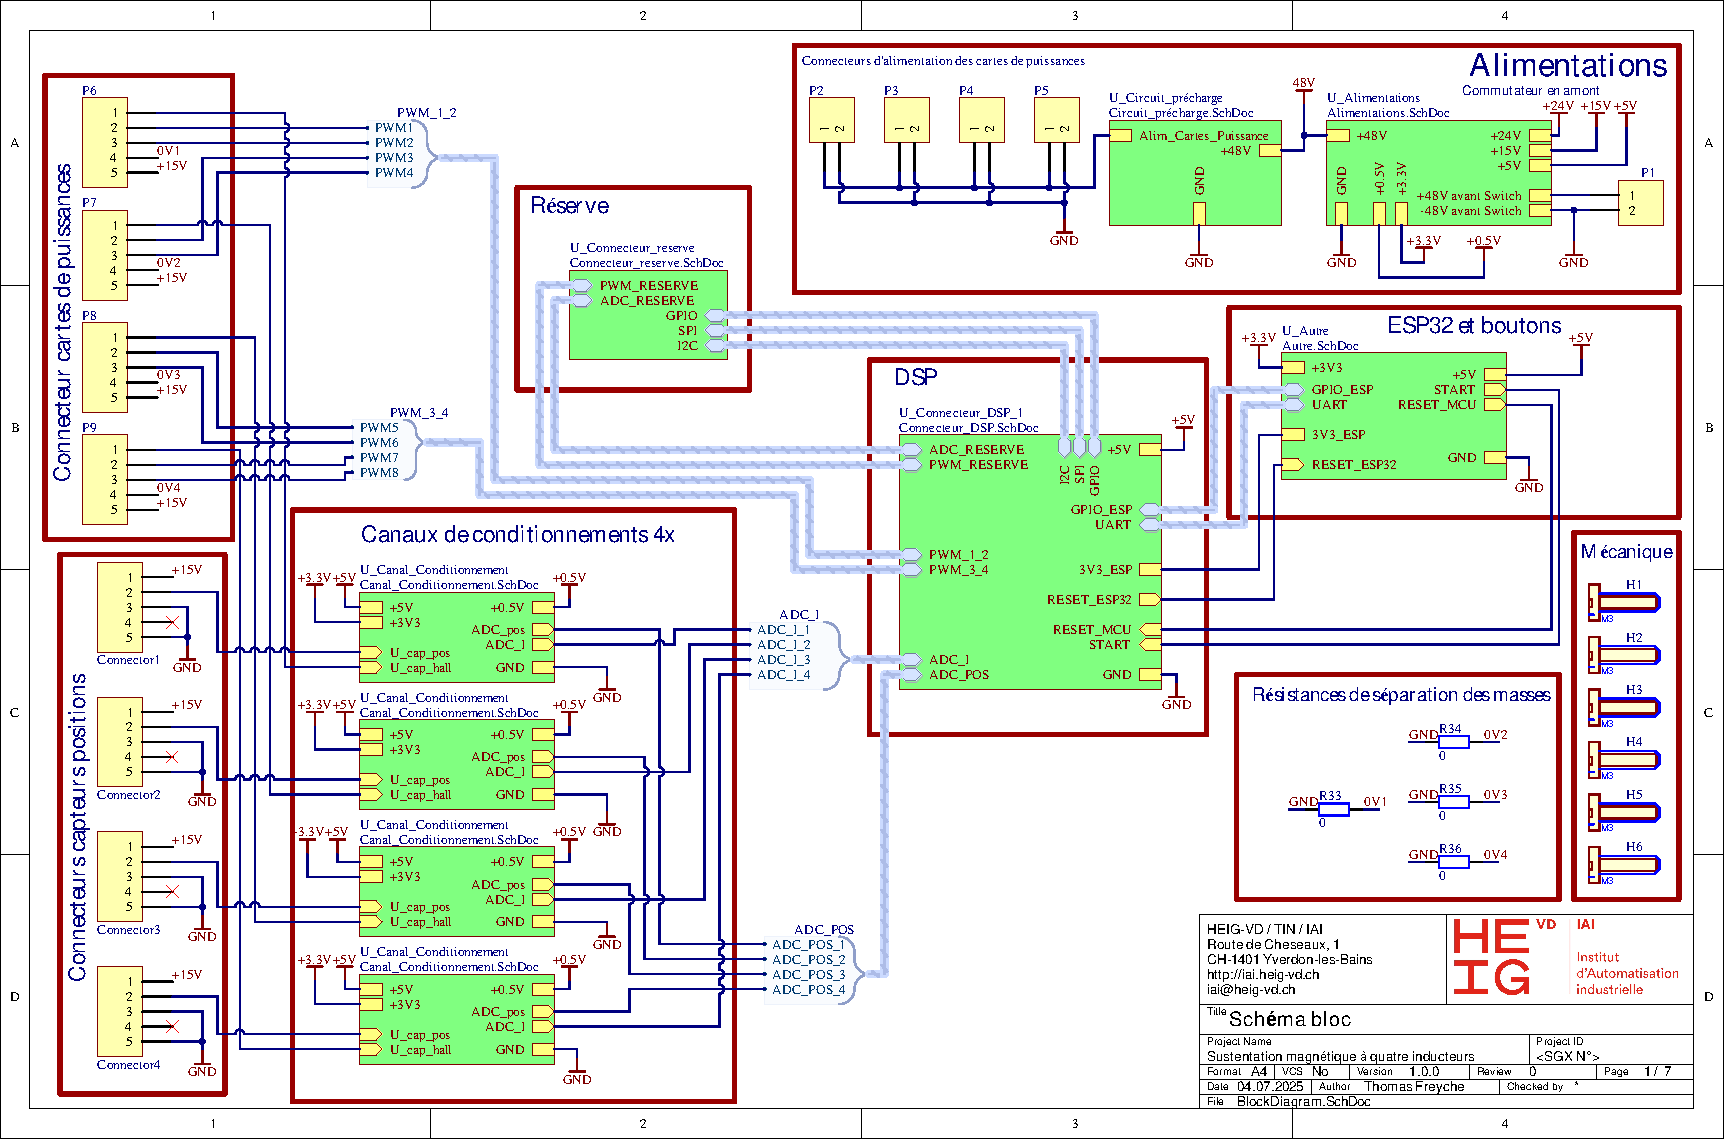
\includegraphics[width=1\linewidth,page=1]{assets/SchemaElectrique/TB_TFE_Sust_Mag_1_0_0.pdf}
    \caption{Schéma électrique \cite{Freyche}}
    \label{fig:SchemaComplet}
\end{figure}

C’est dans cette partie que se situe le cœur de la maquette. On y retrouve :
\begin{itemize}
    \item le DSP exécutant le code de sustentation.
    \item les circuits de conditionnement pour les capteurs de position et de courant.
    \item l’ESP32 pour l’interface web.
    \item l’alimentation des différents éléments de la carte.
    \item les connecteurs pour les cartes de puissance et les capteurs de position.
\end{itemize}

Les sous-sections suivantes présentent les parties décrites ci-dessus.

\subsection{DSP}
Le schéma électrique de l'interface du DSP intègre un connecteur destiné à recevoir une carte d'évaluation Texas Instruments \cite{Freyche}. Cette dernière exécute le programme principal régissant la lévitation. Le connecteur assure ainsi la liaison avec le reste de la carte, comme illustré par la figure \ref{fig:DspScheme} :

\begin{figure}[H]
    \centering
    \includegraphics[page=8, width=1\linewidth]{assets/SchemaElectrique/TB_TFE_Sust_Mag_1_0_0.pdf}
    \caption{Connecteur pour la carte du DSP \cite{Freyche}}
    \label{fig:DspScheme}
\end{figure}

Cette implémentation modulaire permet de retirer facilement la carte d'évaluation en cas de défaillance matérielle du DSP.

Le connecteur et la carte d'évaluation se présentent comme illustré sur la figure \ref{fig:DspEtConnecteur} :

\begin{figure}[H]
    \centering
    % Première sous-figure
    \begin{subfigure}{0.45\textwidth}
        \centering
        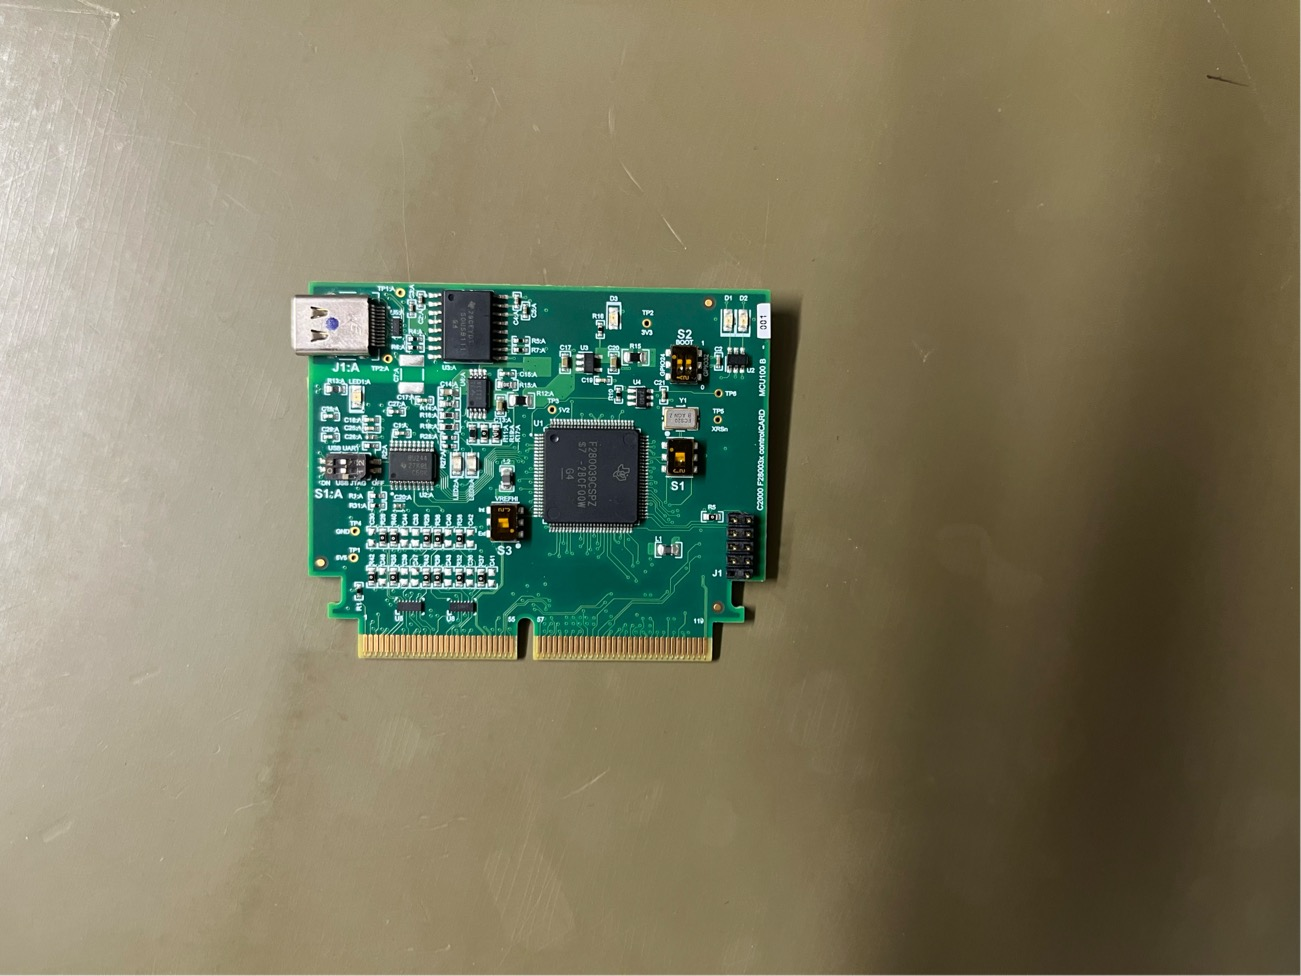
\includegraphics[trim = 80 100 150 80, clip, width=\linewidth]{assets/Chap2/CarteEval.jpg}
        \caption{Carte d'évaluation}
        \label{subfig:carte_eval}
    \end{subfigure}\hfill
    % Deuxième sous-figure
    \begin{subfigure}{0.45\textwidth}
        \centering
        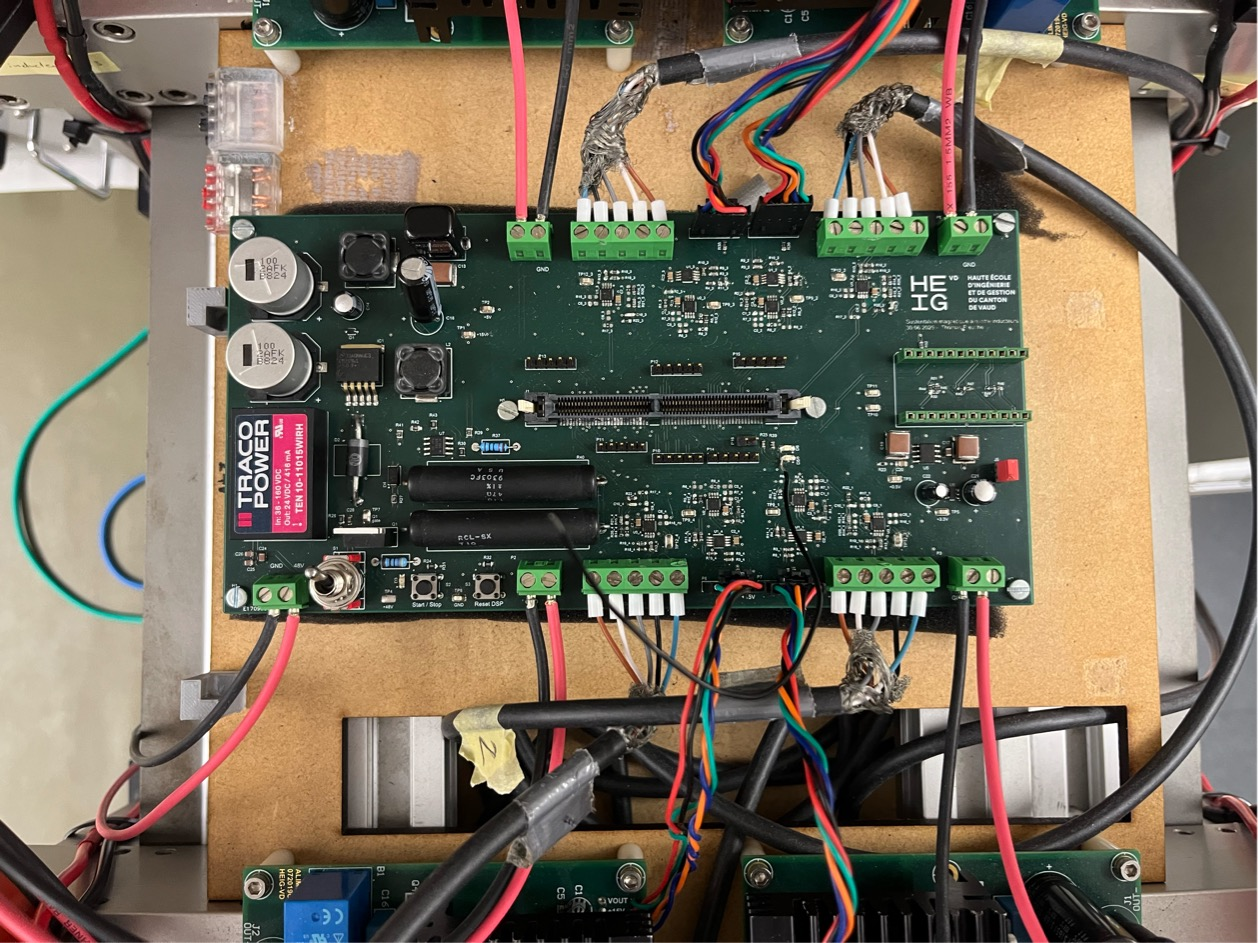
\includegraphics[trim = 50 50 50 50, clip, width=\linewidth]{assets/Chap2/Connector.jpg}
        \caption{Connecteur}
        \label{subfig:connecteur}
    \end{subfigure}

    \caption{Connecteur et carte d'évaluation}
    \label{fig:DspEtConnecteur}
\end{figure}

\subsection{Conditionneurs}
\label{subsec:Conditionneur}
Les conditionneurs permettent de convertir les valeurs brutes des capteurs en signaux exploitables par le microcontrôleur. Cette section se divise en deux parties : la structure supérieure traite le signal du capteur de courant \cite{CaptCour}, tandis que la structure inférieure gère celui du capteur de position \cite{CaptPosition}.

\begin{figure}[H]
    \centering
    \includegraphics[width=1\linewidth,page=4]{assets/SchemaElectrique/TB_TFE_Sust_Mag_1_0_0.pdf}
    \caption{Schéma des conditionneurs de courant et de position \cite{Freyche}}
    \label{fig:ConditionneursScheme}
\end{figure}

Ces circuits permettent d’adapter les tensions mesurées à une plage comprise entre 0 V et 3 V.

Le conditionnement du capteur de courant s’effectue selon les étapes suivantes :
\begin{enumerate}
    \item Le capteur fournit une tension comprise entre 0,625 V et 4,375 V, avec un point milieu à 1,5 V.
    \item Un diviseur de tension d’un facteur 0,8 est réalisé à l’aide de résistances afin de ramener la plage de 0,5 V à 3,5 V.
    \item Un montage à amplificateur opérationnel (AOP) en mode soustracteur est utilisé pour retrancher 0,5 V au signal, afin d’obtenir une plage finale de 0 V à 3 V.
\end{enumerate}

Le conditionnement du capteur de position suit les étapes suivantes :
\begin{enumerate}
    \item Le capteur fournit une tension comprise entre 0 V et 10 V.
    \item Un pont diviseur de tension est appliqué avec un facteur 0,3 pour atteindre une plage de 0 V à 3 V.
\end{enumerate}

L’ensemble des conditionneurs est réalisé de manière identique pour chaque canal de mesure.

La tension de référence de l'ADC étant fixée à 3.3~V, la plage de conversion exploitable est inférieure à la résolution numérique maximale théorique.

La valeur numérique maximale effective est déterminée par un calcul de proportionnalité :

$$3.3\text{ V} = 4095$$
$$3\text{ V} = \text{ADC}_{max}$$

\begin{equation}
    \text{ADC}_{max} = \frac{3}{3,3} \cdot 4095 \approx 3723
    \label{eq:adc_max_calc}
\end{equation}

Cette valeur de crête est ensuite exploitée pour convertir les signaux numériques en grandeurs physiques (courant et position). Les capteur présentant une caractéristique linéaire, leur comportement modélisé s'exprime par une équation du premier degré :

\begin{equation}
    y = ax + b
    \label{eq:droite_lineaire}
\end{equation}

Le calcul du courant s'effectue selon la relation suivante :

$$I = \text{ADC} \cdot \frac{I_{max} - I_{min}}{\text{ADC}_{max}} - I_{offset}$$

Un offset est appliqué au courant afin d'exploiter l'intégralité de la plage de mesure. En effet, sans cette correction, la valeur calculée resterait toujours positive ; en soustrayant l'offset, on retrouve la partie négative de la caractéristique illustrée à la figure \ref{fig:GrapheCaptCour}.

En appliquant les valeurs numériques propres au capteur de courant :

\begin{equation}
    I = \text{ADC} \cdot \frac{30 - (-30)}{3723} - 30 = 0,01612 \cdot \text{ADC} - 30~[\text{A}]
    \label{eq:conv_courant}
\end{equation}

La conversion de la position est simplifiée par l'application d'un étalonnage par apprentissage (\textit{teach-in}) sur le capteur (section \ref{sec:CalibrationCaptPos}). Cette méthode permet de redéfinir la plage de mesure du transducteur : la plage nominale initiale, allant de 30~mm pour 0~V à 70~mm pour 10~V, est ajustée pour correspondre exactement à l'intervalle utile de 0~mm à 3~mm.

La loi de conversion se réduit alors à :

$$\text{Position} = \text{ADC}_{lu} \cdot \frac{\text{Position}_{max} - \text{Position}_{min}}{\text{ADC}_{max}}$$

\begin{equation}
    \text{Position} = \text{ADC} \cdot \frac{3 \cdot 10^{-3} - 0}{3723} = 8,058 \cdot 10^{-7} \cdot \text{ADC}~[\text{m}]
    \label{eq:conv_position}
\end{equation}

\subsection{Alimentation}
Cette section détaille les alimentations des différentes parties de la carte. Les différents blocs sont illustrés sur la figure \ref{fig:AlimSchema} :

\begin{figure}[H]
    \centering
    \includegraphics[width=1\linewidth,page=2]{assets/SchemaElectrique/TB_TFE_Sust_Mag_1_0_0.pdf}
    \caption{Bloc d’alimentation}
    \label{fig:AlimSchema}
\end{figure}

Le système se compose des éléments suivants :
\begin{itemize}
    \item Un convertisseur de tension de 5 V \cite{Reg5V} pour l’alimentation du DSP, de l’ESP32 et de certains AOP. Sa tension d’entrée est de 24 V.
    \item Un convertisseur de 15 V \cite{Reg15V} dédié à l’alimentation des capteurs de position. Sa tension d’entrée est de 24 V.
    \item Un convertisseur permettant d’obtenir une tension de 0,5 V \cite{Reg05V}, utilisée dans le conditionnement des signaux des capteurs de courant.
    \item Un convertisseur de 24 V \cite{Reg24V} utilisé pour alimenter l’ensemble des autres régulateurs. Ce dernier est alimenté par le bus de 48 V. Ce bus est également relié au commutateur permettant l’alimentation des cartes de puissance.
    \item Un convertisseur de 3,3 V \cite{Reg33V} pour l’alimentation de l’ESP32 et de certains AOP. Sa tension d’entrée est de 5 V.
\end{itemize}

Ces composants assurent la distribution des tensions nécessaires au fonctionnement des différents éléments de la carte principale.

\subsection{Circuit de précharge}
Le circuit de précharge a pour objectif d’assurer une mise sous tension progressive des cartes de puissance. Le schéma électrique est présenté sur la figure \ref{fig:PrechSchem}.

\begin{figure}[H]
    \centering
    \includegraphics[width=1\linewidth,page=3]{assets/SchemaElectrique/TB_TFE_Sust_Mag_1_0_0.pdf}
    \caption{Circuit de précharge \cite{Freyche}}
    \label{fig:PrechSchem}
\end{figure}

Le fonctionnement repose sur les étapes suivantes :
\begin{enumerate}
    \item À l’enclenchement, le MOSFET est à l’état bloqué et le courant circule à travers deux résistances de puissance. Celles-ci limitent le courant de charge du condensateur.
    \item Un comparateur confronte la tension aux bornes du condensateur à une tension de référence de 5 V.
    \item Une fois le seuil de tension atteint, le comparateur délivre un signal qui rend le transistor MOSFET passant. Ce dernier court-circuite alors les résistances placées en série, autorisant ainsi l'alimentation directe des cartes de puissance.
\end{enumerate}

\subsection{Cartes de puissance}
Les cartes de puissance sont représentées à la figure \ref{fig:PowerSchem} :

\begin{figure}[H]
    \centering
    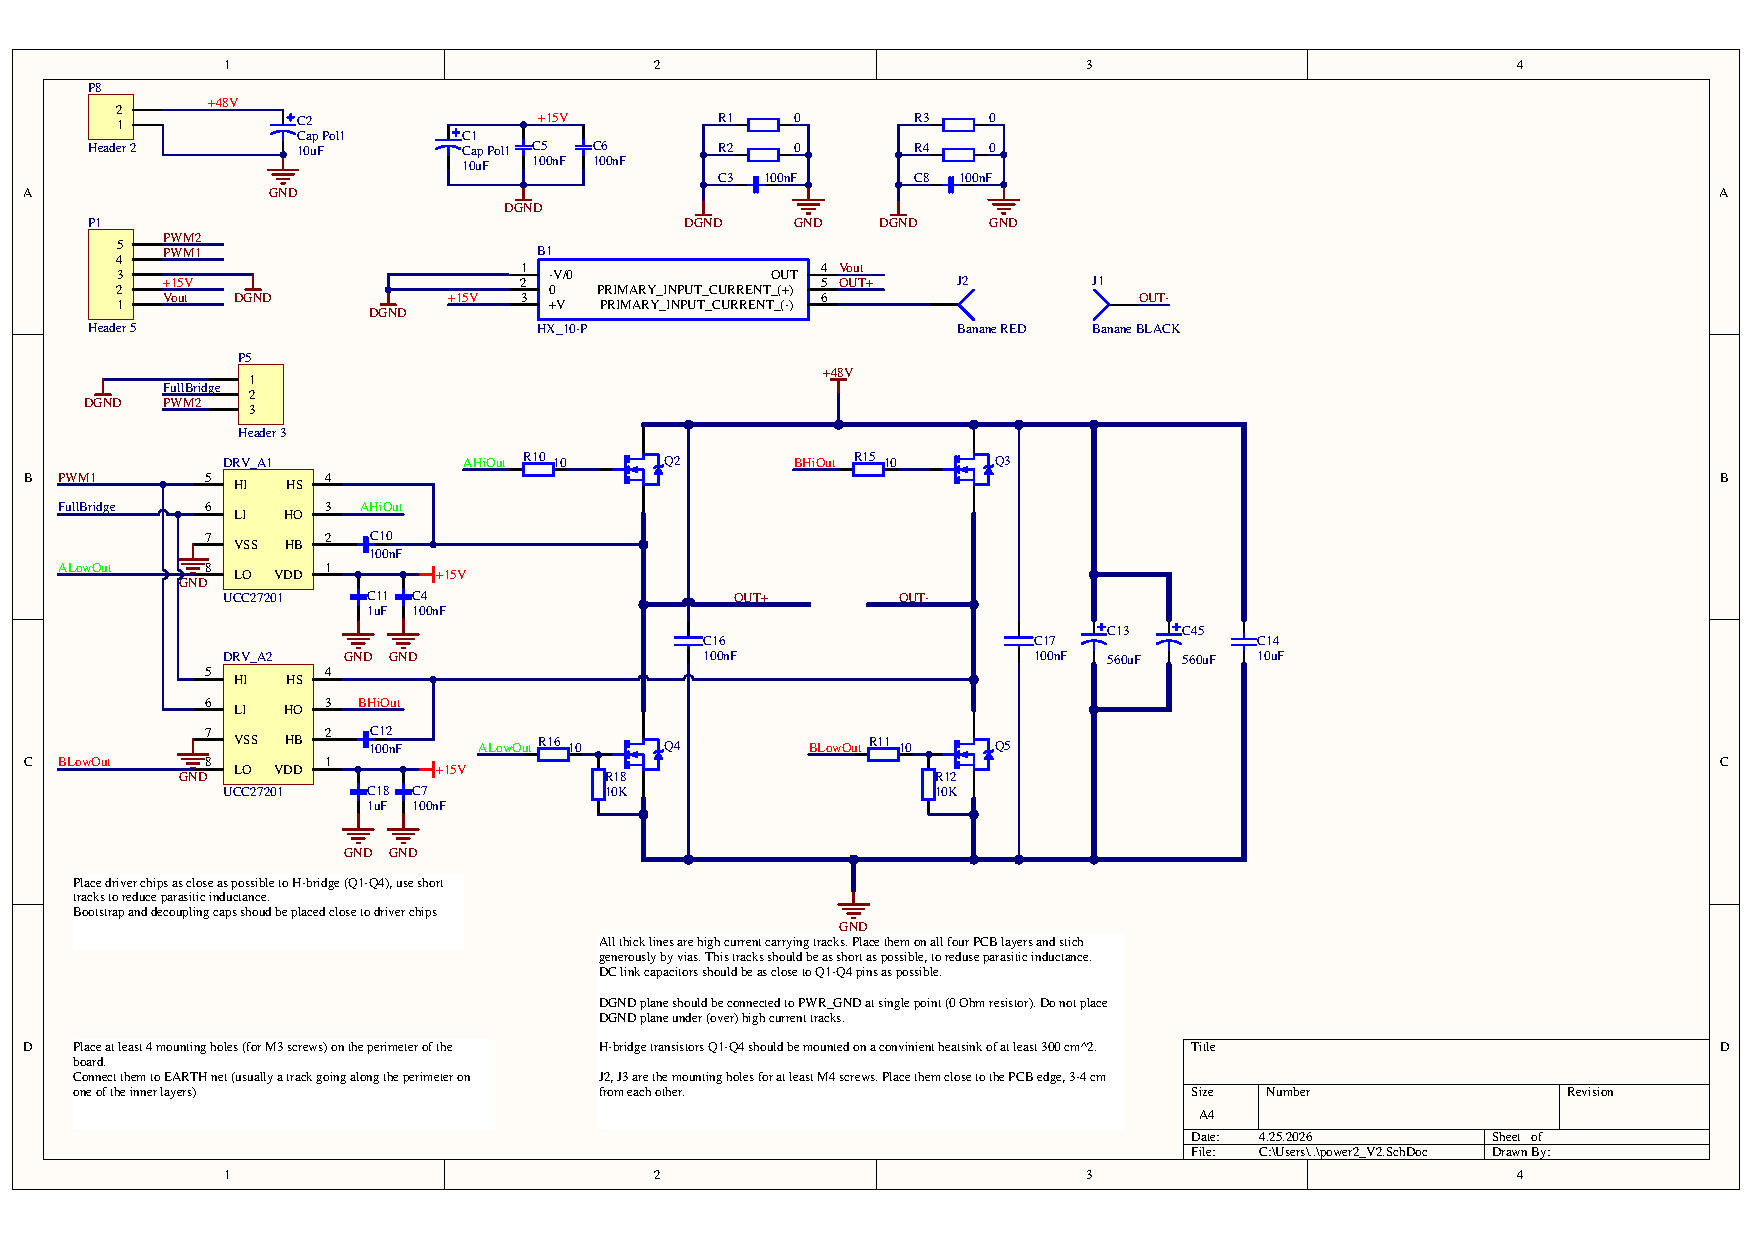
\includegraphics[width=1\linewidth]{assets/SchemaElectrique/power2_V2.pdf}
    \caption{Circuit des cartes de puissance \cite{Laucella}}
    \label{fig:PowerSchem}
\end{figure}

Chaque carte intègre les éléments suivants :
\begin{itemize}
    \item Un pont en H permettant un fonctionnement à 4 quadrants, assurant une circulation bidirectionnelle du courant dans la bobine ainsi qu'un contrôle rapide de sa dynamique (montée/descente).
    \item Deux drivers assurant l’amplification des signaux PWM appliqués sur les MOSFET.
    \item Un capteur de courant destinés à la mesure de l’intensité traversant la bobine.
    \item Des condensateurs de découplage placés en parallèle du bus DC, à proximité du pont en H, afin de garantir la stabilité de la tension d'alimentation face aux appels de courant pulsés du pont.
\end{itemize}

\subsection{ESP32}
L’ESP32 est un microcontrôleur compact utilisé dans ce projet pour fournir une interface web permettant aux utilisateurs d’accéder à diverses informations. Le DSP et l’ESP32 communiquent via une liaison UART afin d’afficher les données sur l’interface web. La carte employée est le modèle Carbon S2, réalisé par GroundStudio \cite{ESP32}.

\begin{figure}[H]
    \centering
    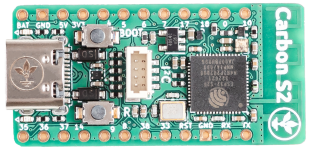
\includegraphics[width=0.5\linewidth]{assets/Chap2/ESP32_Board.png}
    \caption{Carte Carbon S2 \cite{ESP32}}
    \label{fig:Esp32Board}
\end{figure}

D’après la documentation technique \cite{ESP32}, les caractéristiques principales sont les suivantes :
\begin{itemize}
    \item Microcontrôleur : ESP32-S2FN4R2
          \begin{itemize}
              \item[$\ast$] 128 KB de ROM pour le démarrage et les fonctions de base
              \item[$\ast$] 320 KB de SRAM pour les données et instructions
              \item[$\ast$] 16 KB de SRAM RTC
          \end{itemize}
    \item Convertisseur USB-série intégré nativement dans l’ESP32-S2
    \item Régulateur de tension de 3,3 V : ME6211C33U4AG-N
    \item Broches GPIO : 18
    \item Connecteur : USB 2.0 type C
    \item Interfaces : ADC, DAC, contrôleur SD/SDIO/MMC, SPI, EMAC, PWM moteur, PWM LED, UART, I2C, I2S
    \item Fréquence maximale du processeur : 240 MHz
    \item Dimensions approximatives du PCB : 37 mm x 18 mm
\end{itemize}

Le raccordement de la carte est établi selon le schéma \ref{fig:PinoutESP32} :

\begin{figure}[H]
    \centering
    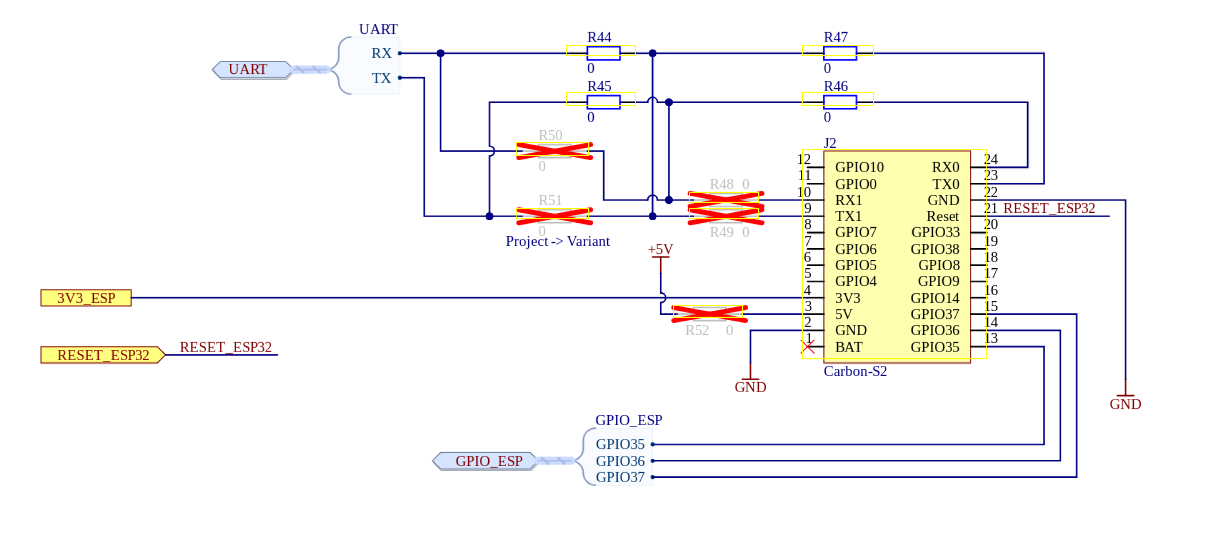
\includegraphics[width=1\linewidth]{assets/Chap2/ESP32_Scheme.png}
    \caption{Schéma de connexion de l’ESP32 \cite{Freyche}}
    \label{fig:PinoutESP32}
\end{figure}

Le schéma définit le brochage suivant :
\begin{itemize}
    \item les broches 24 et 23 (TX/RX) pour la communication UART.
    \item l’alimentation sur la broche 4 (3,3 V) et les broches 2 et 22 (GND).
    \item le reset sur la broche 23.
    \item les signaux MISO, MOSI et SCK sur les broches 13, 14 et 15.
\end{itemize}